% 建议使用 XeLaTeX 或 LuaLaTeX 编译(中文与公式支持更佳)
\documentclass[UTF8,zihao=-4]{ctexart}

\usepackage[a4paper,margin=2.5cm]{geometry}
\usepackage{amsmath, amssymb, amsthm}
\usepackage{bm}
\usepackage{hyperref}
\usepackage{graphicx}
\usepackage{caption}
\usepackage{listings}
\usepackage{xcolor}
\usepackage{float}
\usepackage{placeins}
\graphicspath{{figures/}}

\lstdefinestyle{code}{
  basicstyle=\ttfamily\small,
  numbers=left,
  numberstyle=\tiny,
  numbersep=8pt,
  keywordstyle=\color{blue},
  commentstyle=\color{teal!70!black},
  stringstyle=\color{orange!70!black},
  showstringspaces=false,
  breaklines=true,
  frame=single,
  framerule=0.3pt,
  rulecolor=\color{black!15}
}
\lstset{style=code}

\title{DBSCAN:原理、公式、应用与实战}
\author{}
\date{\today}

\begin{document}
\maketitle

\section{引言}
DBSCAN(Density-Based Spatial Clustering of Applications with Noise)通过密度连接来发现任意形状的簇,并天然识别噪声点。算法由邻域半径 \(\varepsilon\) 与核心点阈值 \(\texttt{minPts}\) 控制:只要在 \(\varepsilon\) 邻域内至少包含 \(\texttt{minPts}\) 个点,就视为高密度区域,从而扩展出簇。相比需要预先设定簇数量的算法(如 K-means),DBSCAN 更擅长处理不规则边界与离群点,但在簇密度差异较大时需要谨慎调参。

\section{原理与公式}
\subsection{邻域与核心点}
任意样本点 \(p\) 的 \(\varepsilon\) 邻域可写为
\begin{equation}
\mathcal{N}_\varepsilon(p) = \{ q\mid \lVert p - q \rVert_2 \le \varepsilon \}.
\end{equation}
若 \(|\mathcal{N}_\varepsilon(p)| \ge \\texttt{minPts}\),则称 \(p\) 为核心点;处于核心点邻域中但自身非核心的点为边界点;仍未被分配的则标记为噪声。

\subsection{密度可达与密度相连}
若 \(p\) 为核心点且 \(q \in \mathcal{N}_\varepsilon(p)\),则称 \(q\) 对 \(p\) 密度直接可达。沿核心点链传递即可得到密度可达性:
\begin{equation}
q \text{ 对 } p \text{ 密度可达} \iff \exists \; p = p_0, p_1, \dots, p_k = q, \; p_{i+1} \in \mathcal{N}_\varepsilon(p_i).
\end{equation}
簇被定义为一组互相密度相连的点的最大集合,并至少含有一个核心点。

\subsection{算法流程}
\begin{enumerate}
  \item 预处理与特征缩放,确保距离度量具有实际意义。
  \item 遍历样本,若某点未访问则计算其 \(\mathcal{N}_\varepsilon(p)\)。当点不是核心点时临时视作噪声。
  \item 对核心点创建新簇,并将邻域内所有点纳入;若邻居也是核心点,则继续扩张。
  \item 重复上述过程直至所有点被划分为簇或噪声。
\end{enumerate}
常用欧氏距离,但在稀疏或文本场景可改用余弦距离等度量。

\section{应用与技巧}
\begin{itemize}
  \item \textbf{地理空间聚类}:定位交通热点、犯罪高发区或商圈密集区,不需预设簇数。
  \item \textbf{异常检测}:噪声点可视为离群事件,例如传感器故障或异常交易。
  \item \textbf{参数选择}:利用 k 距离曲线(通常 \(k = \texttt{minPts}-1\))寻找“肘点”估计 \(\varepsilon\),并根据维度经验先设 \(\texttt{minPts} = 2d\)。
  \item \textbf{数据准备}:数值特征需标准化,删除重复点;高维数据可先降维以提升查询效率与密度判断稳定性。
\end{itemize}

\section{Python 实战}
脚本 \texttt{gen\_clustering\_dbscan\_figures.py} 构造三个致密簇与噪声点,并基于 \(\varepsilon=0.35\)、\(\texttt{minPts}=5\) 运行 DBSCAN;同时计算第 \(k\) 近邻距离序列帮助挑选参数。
\begin{lstlisting}[language=Python,caption={脚本 gen_clustering_dbscan_figures.py 片段}]
dbscan = DBSCAN(eps=0.35, min_samples=5, metric="euclidean")
labels = dbscan.fit_predict(points)

neighbors = NearestNeighbors(n_neighbors=5)
dists, _ = neighbors.kneighbors(points)
ordered = np.sort(dists[:, -1])
\end{lstlisting}

\section{实验结果}
\begin{figure}[H]
  \centering
  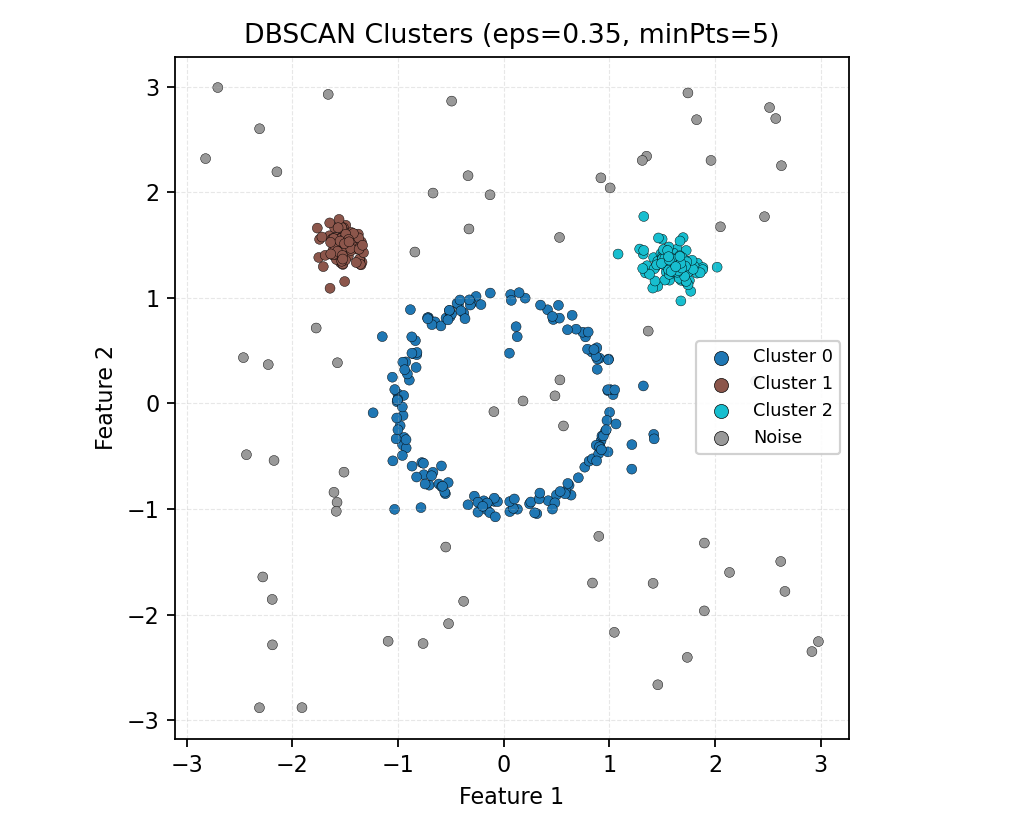
\includegraphics[width=0.82\linewidth]{dbscan_clusters.png}
  \caption{DBSCAN 在含噪声的合成数据上得到的聚类结果}
  \label{fig:dbscan_clusters_cn}
\end{figure}

\begin{figure}[H]
  \centering
  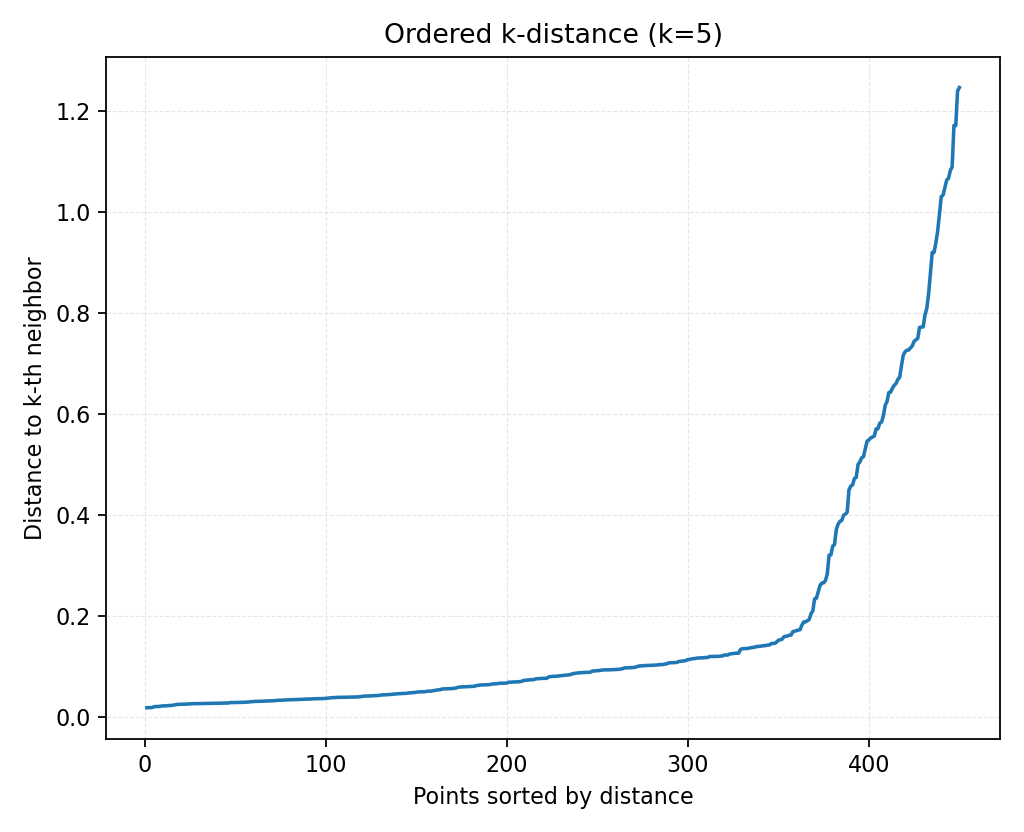
\includegraphics[width=0.82\linewidth]{dbscan_k_distance.png}
  \caption{第五近邻距离曲线在 \(\varepsilon\approx0.35\) 附近出现显著弯折}
  \label{fig:dbscan_k_distance_cn}
\end{figure}

\FloatBarrier
\section{总结}
DBSCAN 能够在未知簇数的情况下挖掘任意形状的密集区域,并对稀疏区域标记噪声。实践时应关注距离度量、缩放方式以及 \(\varepsilon\) 与 \texttt{minPts} 的协同调节;借助 k 距离曲线与可视化可以快速验证参数合理性。

\end{document}

